\documentclass[border=5pt]{standalone}
\usepackage{amsmath}
\usepackage{tikz}
\usetikzlibrary{arrows.meta,decorations.markings}
\begin{document}
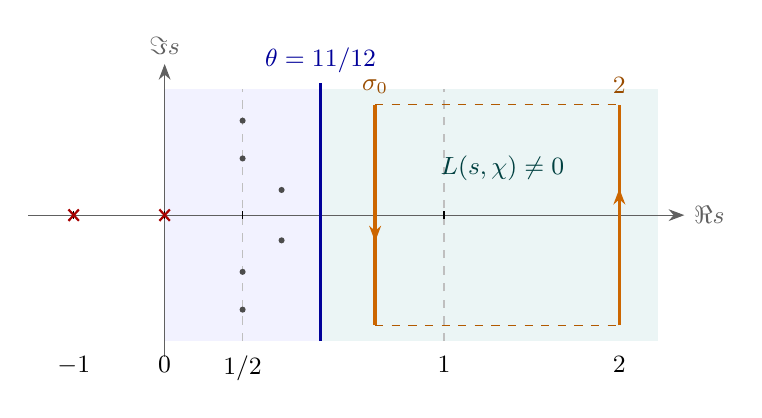
\begin{tikzpicture}[x=1.65cm,y=0.8cm,>={Stealth[length=2mm]},font=\small]
\fill[blue!5] (-0.5,-2)--(0.7,-2)--(0.7,2)--(-0.5,2)--cycle;
\fill[teal!8] (0.7,-2)--(3.3,-2)--(3.3,2)--(0.7,2)--cycle;
\draw[->,gray!75!black] (-1.55,0)--(3.5,0) node[right]{$\Re s$};
\draw[->,gray!75!black] (-0.5,-2.25)--(-0.5,2.4) node[above]{$\Im s$};
\draw[blue!60!black,thick] (0.7,-2)--(0.7,2.1)
 node[above,align=center]{$\theta=11/12$};
\draw[gray!50,dashed] (0.1,-2)--(0.1,2);
\draw[gray!50,dashed] (1.65,-2)--(1.65,2);
\foreach \x/\label in {-1.2/{-1},-0.5/0,0.1/{1/2},1.65/1,3/2}
 {\draw (\x,0.06)--(\x,-0.06);\node[below] at (\x,-2.08) {$\label$};}
\foreach \x in {-1.2,-0.5}
 {\draw[red!65!black,thick] (\x-0.04,-0.09)--(\x+0.04,0.09)
 (\x-0.04,0.09)--(\x+0.04,-0.09);}
\foreach \x/\y in {0.1/1.5,0.1/0.9,0.1/-0.9,0.1/-1.5,0.4/0.4,0.4/-0.4}
 {\fill[black!70] (\x,\y) circle (1.1pt);}
\draw[orange!80!black,very thick,postaction={decorate},
 decoration={markings,mark=at position .62 with {\arrow{>}}}]
 (3,-1.75)--(3,1.75);
\draw[orange!80!black,very thick,postaction={decorate},
 decoration={markings,mark=at position .62 with {\arrow{>}}}]
 (1.12,1.75)--(1.12,-1.75);
\draw[orange!70!black,dashed] (1.12,-1.75)--(3,-1.75)
 (1.12,1.75)--(3,1.75);
\node[orange!60!black,above,align=center] at (1.12,1.78) {$\sigma_0$};
\node[orange!60!black,above] at (3,1.78) {$2$};
\node[teal!50!black,align=center] at (2.1,.75) {$L(s,\chi)\ne0$};
\end{tikzpicture}
\end{document}
